\documentclass[12pt]{ctexart}

\usepackage{amsmath}
\usepackage{booktabs}
\usepackage{graphicx}

\title{数据分析报告}
\author{Jack}
\date{}

\begin{document}

\maketitle

\section{样本数据呈现}

将原始数据可视化,如表~\ref{tab:rawdata} 所示

\begin{table}
    \centering
    \caption{样本数据}
    \label{tab:rawdata}
    \begin{tabular}{cccc}
\toprule
temperature & sales & humidity & cost \\
\midrule
20 & 100 & 80 & 50 \\
22 & 120 & 75 & 55 \\
25 & 145 & 70 & 60 \\
27 & 160 & 65 & 68 \\
30 & 190 & 60 & 75 \\
32 & 210 & 55 & 82 \\
\bottomrule
\end{tabular}

\end{table}

\section{数据分析}

本文对样本数据进行初步可视化分析。

\subsection{散点图分析}

样本散点分布如图~\ref{fig:scatter} 所示。

\begin{figure}[htbp]
    \centering
    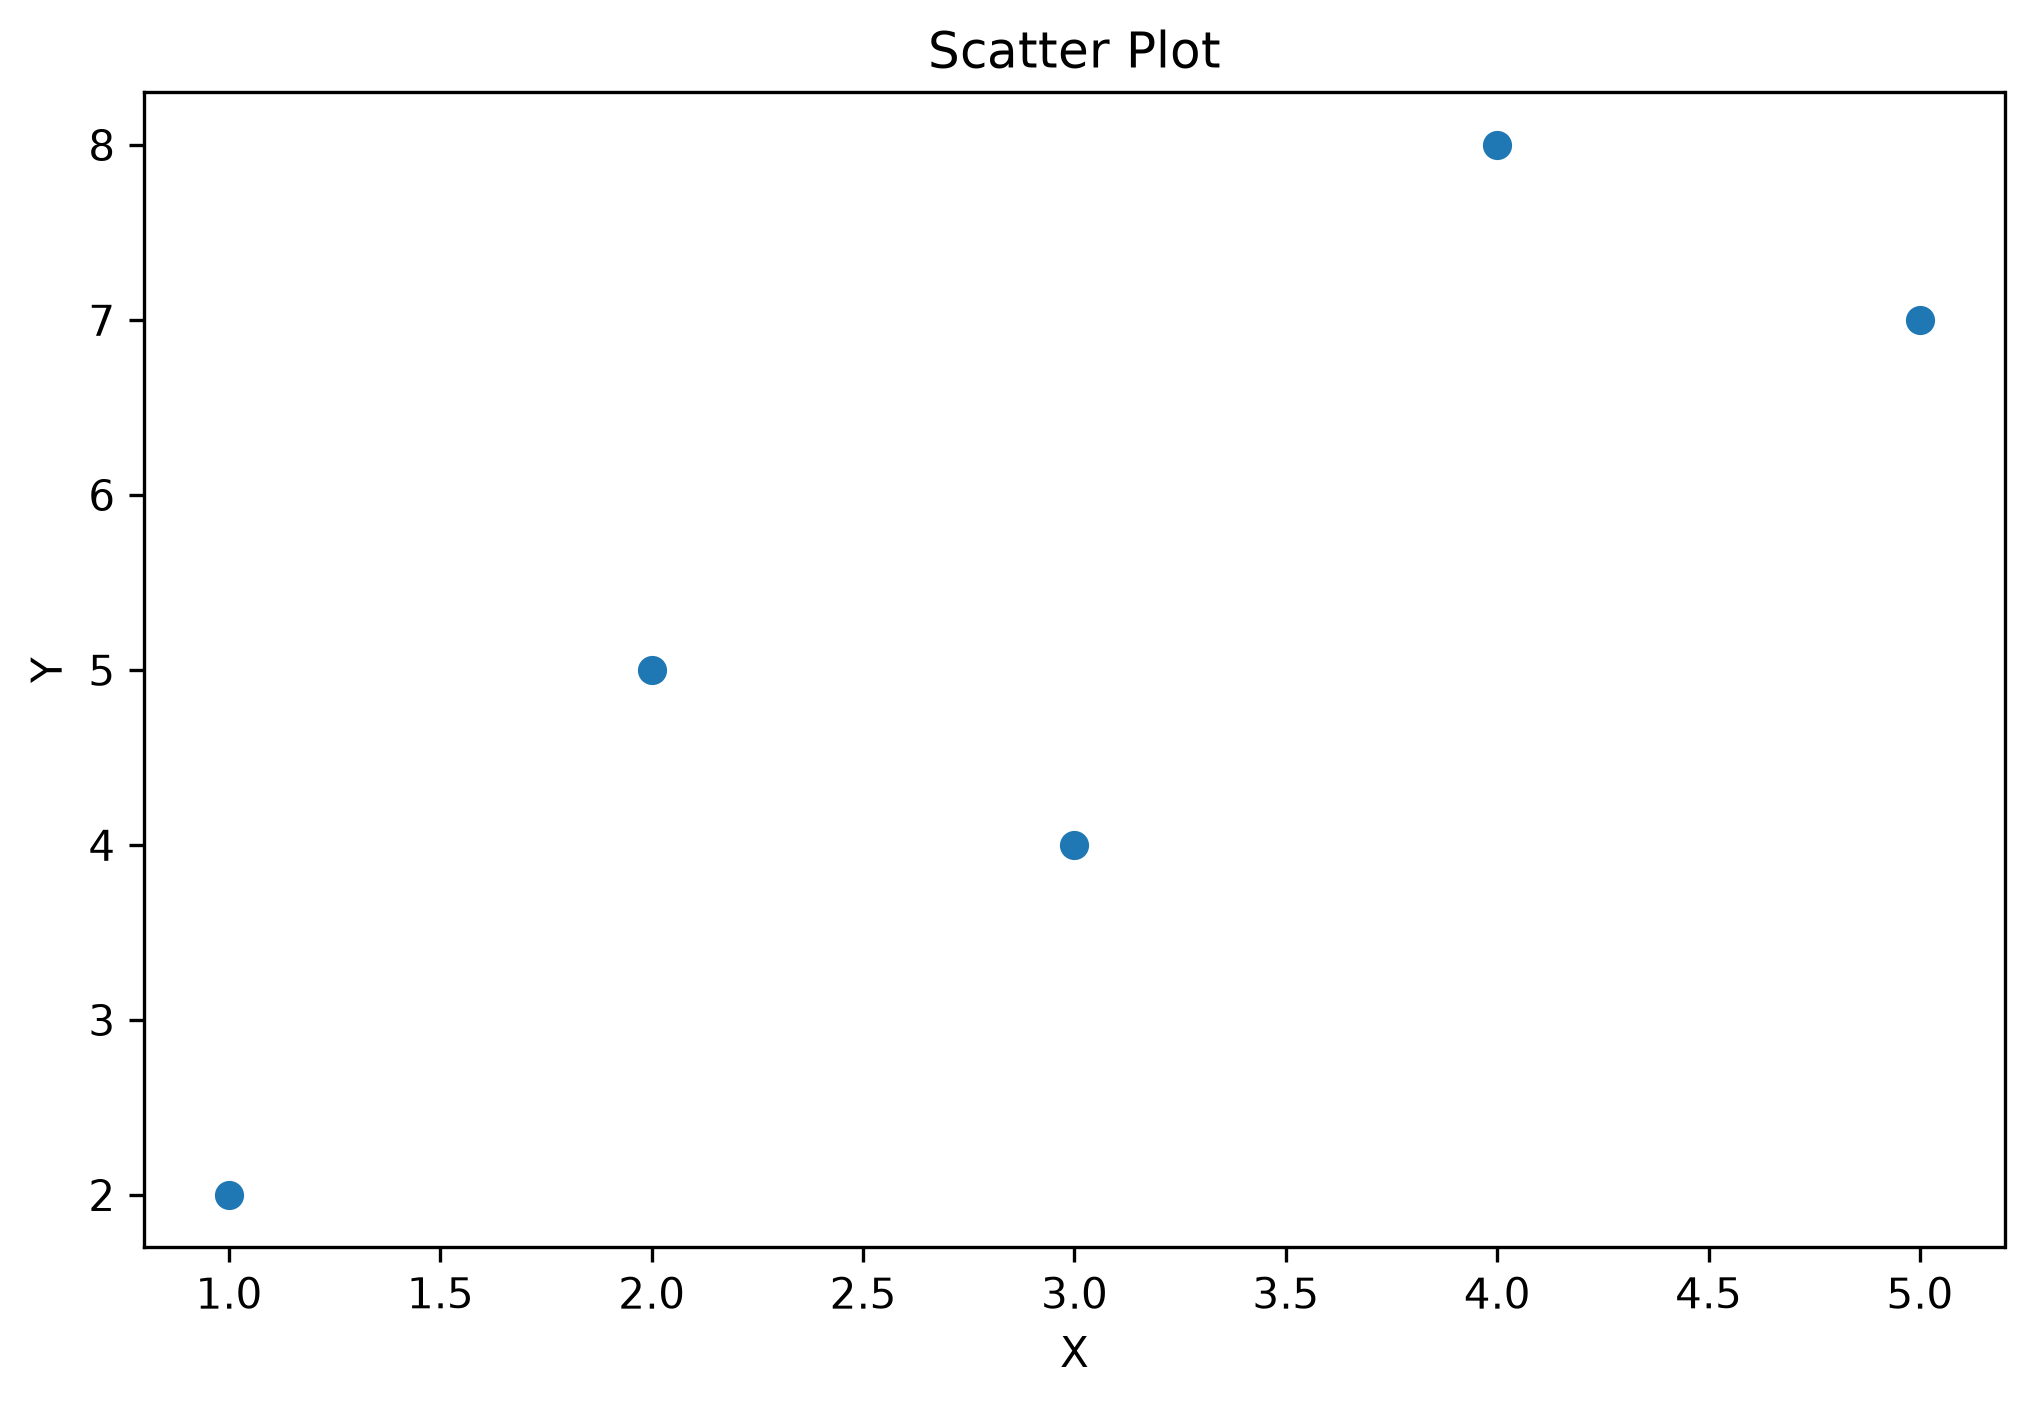
\includegraphics[width=0.7\textwidth]{../../figures/scatter.png}
    \caption{散点图}
    \label{fig:scatter}
\end{figure}

\subsection{数据相关性分析}

Pearson 相关系数定义为

\begin{equation}
    r_{XY}
    =
    \frac{\operatorname{cov}(X,Y)}
    {\sigma_X\sigma_Y}.
    \label{eq:pearson}
\end{equation}

由式~\ref{eq:pearson} 计算各变量之间的线性相关关系，其结果如图~\ref{fig:corr} 所示。

\begin{figure}[htbp]
    \centering
    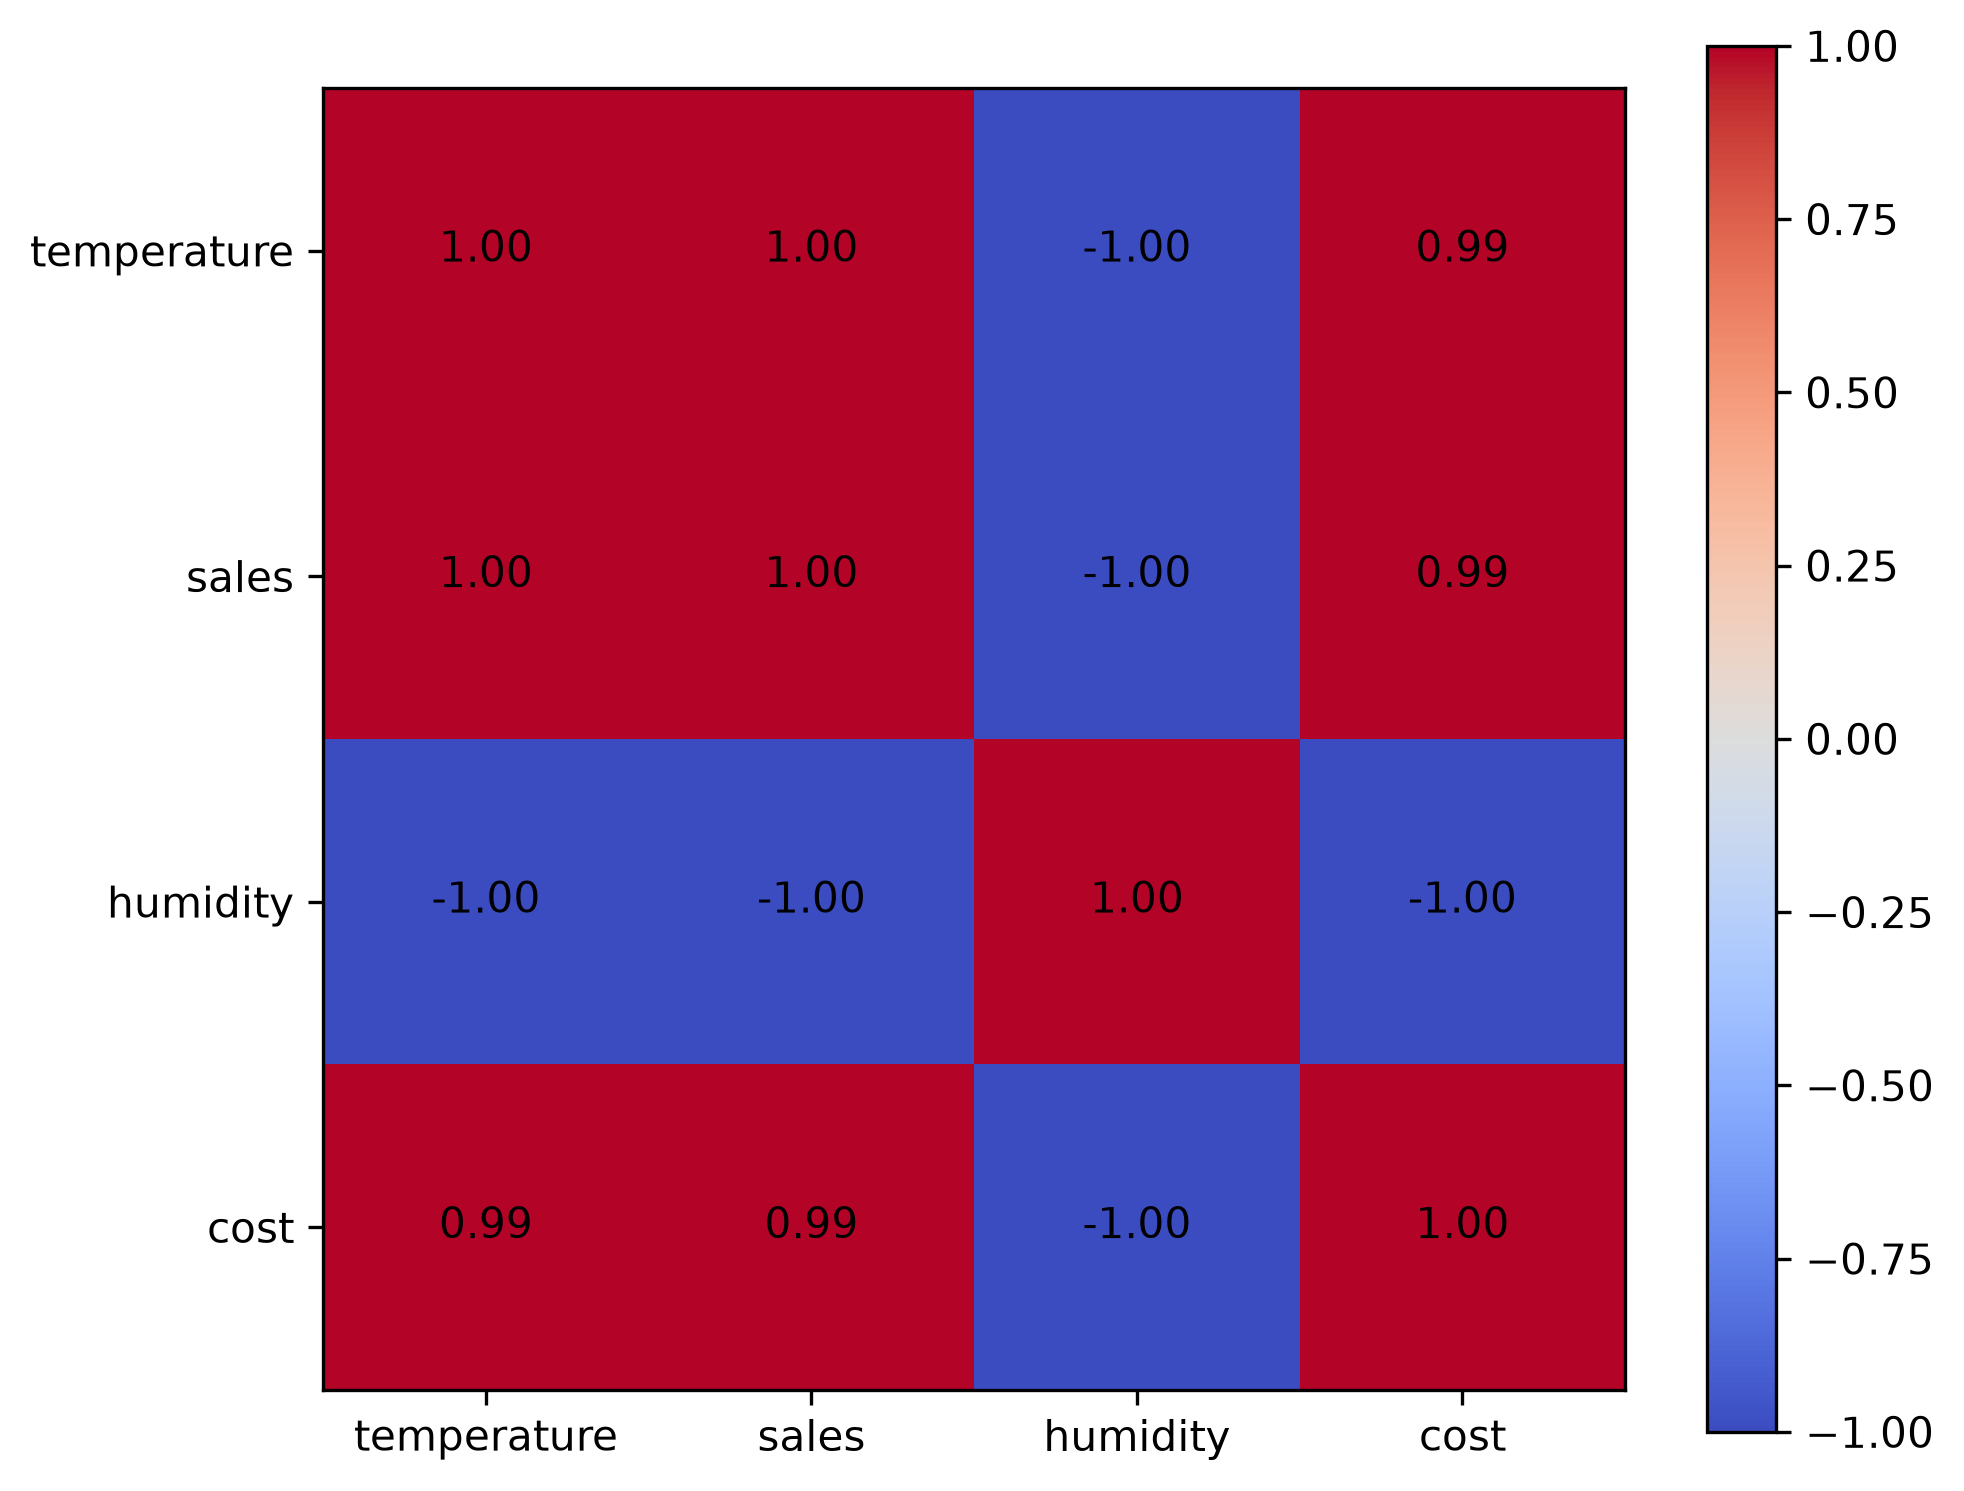
\includegraphics[width=0.7\textwidth]{../../figures/correlation_heatmap.png}
    \caption{热力图}
    \label{fig:corr}
\end{figure}




    
\end{document}